\subsection{Celdas de Combustible}

A pesar de que las celdas de combustible son una tecnología de hace más de un siglo y medio (desarrollada por primera vez por el físico galés Sir William Grove en 1842), hoy en día despiertan un particular interés en el campo de la generación renovable por su alta eficiencia, su dependencia en recursos obtenibles fácilmente de maneras ambientalmente amigables, y por la generación de agua como único deshecho.\\

Por estas razones se eligió trabajar con esta tecnología, particularmente con el tipo de celda más común hoy en día, las Celdas de Combustible de Membrana de Intercambio Protónico o PEMFC (del inglés \textit{Proton Exchange Membrane Fuel Cell}), cuyo funcionamiento se profundiza más adelante.\\

\subsubsection{Principio de Funcionamiento de las Celdas de Combustible}

Esencialmente, una celda de combustible es una celda galvánica o celda voltáica en la cual la energía libre de una reacción química redox (entre un combustible y un agente oxidante o \textit{comburente}) se convierte a energía eléctrica mediante una corriente y una diferencia de potencial$^{[FC-FundamentalsAndApplications]}$. En nuestro caso particular, el combustible es el hidrógeno molecular ($H_2$), el agente oxidante es el oxígeno ($O_2$) abundante en la atmósfera, y los productos son la energía eléctrica y el agua ($H_2O$) según indica la siguiente ecuación química balanceada.

\begin{equation}\label{redox_celda}
    H_2\ +\ \frac{1}{2}O_2\ \longrightarrow\ H_2O
\end{equation}

La estructura interna de una celda de combustible, visible en la figura \ref{fuel_cell}, consiste de un ánodo (electrodo negativo) al cual ingresan las moléculas de hidrógeno, un cátodo (electrodo positivo) en el que ingresa el oxígeno y se despide el agua, y un electrolito como como interfaz entre ánodo y cátodo. La carga es conectada entre el ánodo y el cátodo.

\begin{figure}[h]
    \centering
    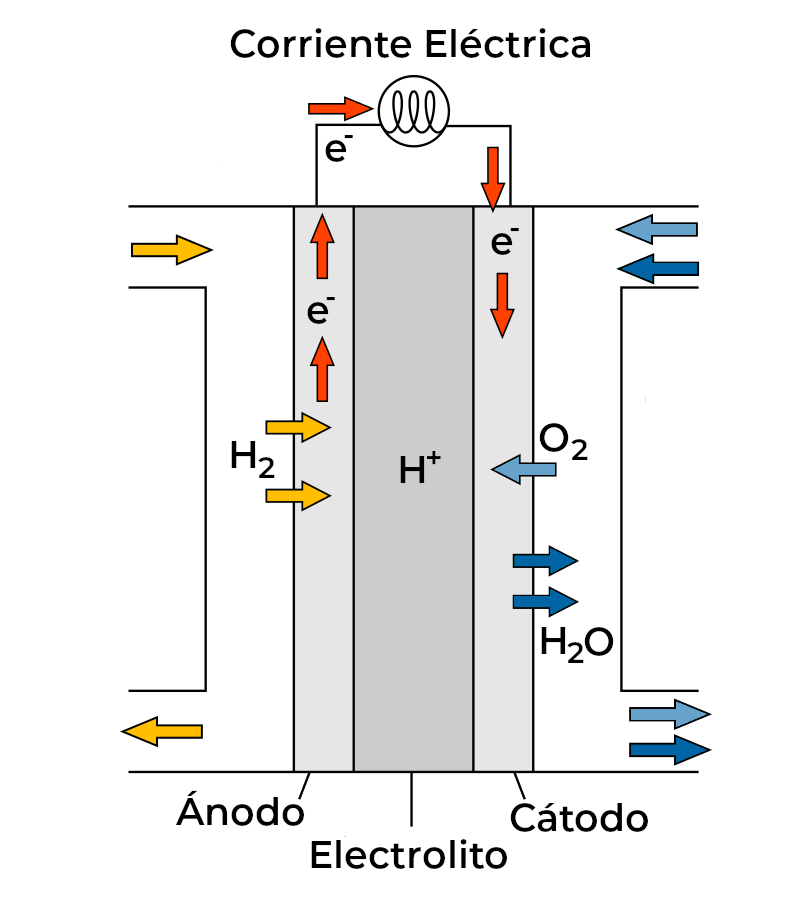
\includegraphics[scale=0.35]{Imagenes/Fuel Cell.png}
    \caption{Esquema de una celda de combustible, con todos sus componentes indicados (Placeholder).}
    \label{fuel_cell}
\end{figure}

La reacción redox de la ecuación \ref{redox_celda}, dentro de una celda de combustible como la del esquema, en realidad se separa en dos reacciones parciales distintas:

\begin{equation}\label{redox_anodo}
    H_2\ \longrightarrow\ 2H^{+}\ +\ 2e^-
\end{equation}

\begin{equation}\label{redox_catodo}
    2H^{+}\ +\ 2e^-\ +\ \frac{1}{2}O_2\longrightarrow\ H_2O
\end{equation}

De esta manera, alimentado simultáneamente el terminal negativo con combustible (hidrógeno) y el terminal positivo con oxidante (oxígeno) se producen las dos reacciones en las superficies de contacto del electrolito:

\begin{itemize}
    \item \textbf{En el ánodo ocurre la oxidación:} las moléculas de $H_2$ pierden sus electrones, bifurcándose los iones positivos de hidrógeno ($H^{+}$) por el electrolito y los electrones libres a través de la carga (ecuación \ref{redox_anodo}). Es una reacción exotérmica (libera calor) que resulta en el calentamiento de la celda.
    \item \textbf{En el cátodo ocurre la reducción:} los iones $H^{+}$ del electrolito, los electrones libres, y las moléculas de oxígeno reaccionan para formar como producto el agua (ecuación \ref{redox_catodo}).
\end{itemize}

Mediante este proceso electroquímico se generan dos corrientes distintas: una corriente interna de iones $H^{+}$ (cargas positivas) en el electrolito, desde el ánodo hacia el cátodo; y una corriente externa de electrones $e^-$ (cargas negativas) circulando por la carga, en el mismo sentido que la corriente de iones. Esta última corriente de electrones es la que nos resulta útil para poder alimentar algún tipo de carga.\\

\subsubsection{De Celda a Pila de Combustible}

Sin embargo, una celda de combustible individual como en la figura \ref{fuel_cell} no es capaz de entregar una diferencia de potencial lo suficientemente alta para la gran mayoría de las aplicaciones, con una tensión de celda común situada entre \SI{0.7}{\volt} y \SI{1.3}{\volt}, dependiendo de varios aspectos constructivos específicos de la celda.\\

Entonces, para obtener un dispositivo con una tensión de salida de niveles utilizables, esta tecnología generalmente se comercializa en forma de pilas o \textit{stacks} de celdas individuales conectadas en serie como se ve en la figura \ref{fuel_cell_stack}, generalmente de entre diez y cien celdas, cuya tensión es la suma de la tensión de cada celda que la compone.\\

Esto se logra, como dice su nombre, apilando todas las celdas de combustible para formar el \textit{stack}, utilizando placas de interconexión para conectar electrodos de polaridad opuesta de dos celdas aledañas (es decir, se conecta el ánodo de una celda con el cátodo de la siguiente); además de cumplir la función de aislar el combustible de una celda del agente oxidante de la celda contigua. Este es el tipo de conexionado de celdas más común, llamado \textit{Planar-Bipolar Stacking} o Apilado Planar-Bipolar$^{[FCHandbook]}$.

\begin{figure}[H]
    \centering
    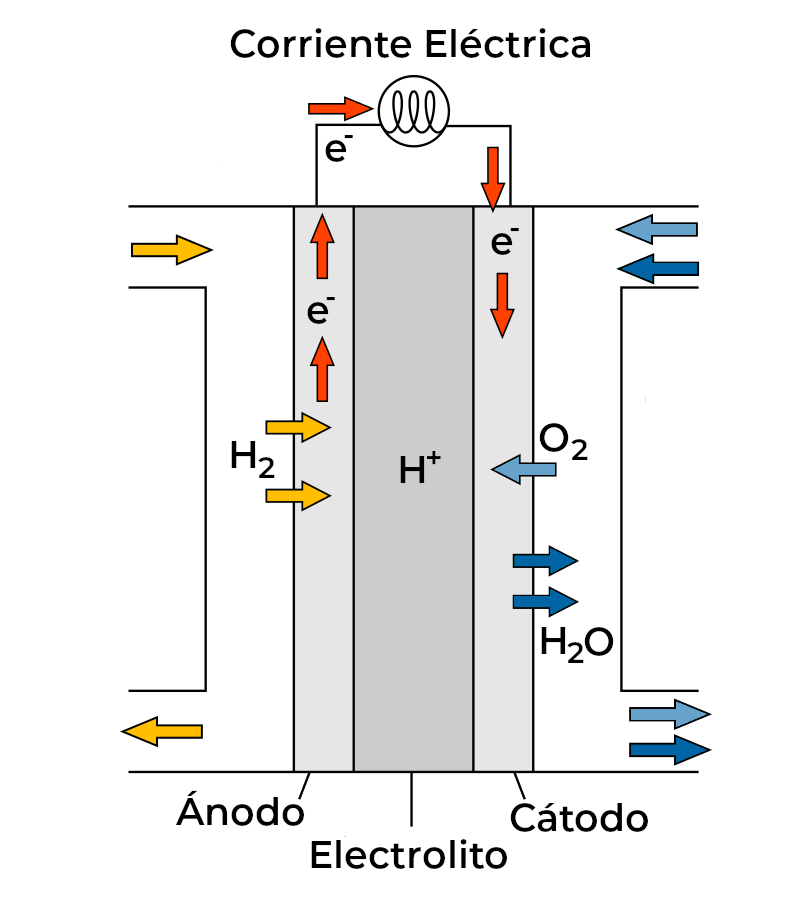
\includegraphics[scale=0.2]{Imagenes/Fuel Cell.png}
    \caption{Figura de un stack de celdas.}
    \label{fuel_cell_stack}
\end{figure}

\subsubsection{Aspectos Constructivos de Celdas}

Habiendo repasado el principio básico de funcionamiento de las celdas de combustible, ahora se realizará una breve descripción de los aspectos constructivos de las mismas. La utilización de distintos materiales y composiciones de las partes que las componen derivan en distintos tipos de celdas, que, a pesar de funcionar bajo el mismo principio básico, poseen cada una sus ventajas y desventajas que las hacen más o menos apropiadas para distintas aplicaciones.\\

Como las reacciones químicas ocurren en superficies microscópicas dónde alguno de los electrodos está en contacto con el electrolito, generalmente los electrodos se fabrican de materiales porosos que aumentan la posible superficie de contacto entre ambas fases, acelerando las reacciones necesarias para producir energía. Sin embargo, en muchos casos, a temperaturas bajas los materiales de los electrodos no son capaces de producir la suficiente actividad electroquímica, por lo que suelen agregarse pequeñas cantidades de catalizador en las zonas de contacto para acelerar la reacción.\\

En tanto al electrolito, estos suelen estar hechos de materiales en estado líquido o sólido, dependiendo del tipo de celda, pero siempre deben tener una alta conductividad de iones positivos, de manera que los iones $H^{+}$ circulen solo por el elctrolito y no por el circuito externo. Adicionalmente, este material debe actuar de barrera física para evitar que se mezclen los flujos de combustible y comburente.\\

En tanto a la geometría de las celdas, se ha expermientado con una gran variedad de formas para los electrodos y electrolitos pero, hoy en día las pilas que se producen son mayormente planas, y en algunos casos tubulares.\\

\subsubsection{Tipos de Celdas}\label{tipos_celdas}

Hay muchas formas de clasificar las distintas tecnologías de celdas, pero en nuestro caso nos vamos a enfocar en la distinción más común, que es la clasificación según el material usado como electrolito. Hoy en día, hay seis tipos distintos de celdas segun electrolito, descritas a continuación, con una mayor profundización mayor en las del tipo PEMFC que se mencionaron anteriormente, ya que son este tipo de pilas las que nos interesa en nuestra aplicación particular.\\

\begin{itemize}
    \item \textbf{Celda de Combustible Alcalina (AFC)}\\
    Las AFC fueron las primeras celdas de combustible en ser desarrolladas, alrededor de 1960, e incluso hoy en día son las celdas de combustible con la mayor eficiencia eléctrica. Sin embargo, resultan poco viables, principalmente porque requieren gases muy puros para funcionar correctamente. Este requerimiento se da por el material electrolítico utilizado, el Hidróxido de Potasio (KOH) (en concentraciones de \SI{85}{\percent} para celdas de alta temperatura (\SI{250}{\celsius}), y entre \SI{35}{\percent} y \SI{50}{\percent} para celdas de baja temperatura (<\SI{120}{\celsius})), que reacciona facilmente con el dióxido de carbono que abunda en el aire, transformándose en $K_2CO_3$, destruyendo el electrolito y la celda en el proceso$^{[FCHandbook][FCCarrette]}$.\\

    \item \textbf{Celda de Combustible de Membrana de Intercambio Protónico (PEMFC)}\\
    Las PEMFC, también llamadas Celdas de Combustible de Electrolito Polimérico Sólido (SPEFC) son las celdas de combustible más utilizadas al día de hoy, habiendo conseguido usos en vehículos de combustible alternativo, lo que resultó en una gran inversión para su desarrollo. Estas celdas operan en rangos bajos de temperatura (entre \SI{65}{\celsius} y \SI{105}{\celsius}) y tienen un electrolito de estado sólido.\\
    
    Este electrolito es una membrana de intercambio protónico: un membrana semipermeable que permite la conducción de protones y al mismo tiempo funcionando de aislación eléctrica entre los electrodos, y como barrera física para separar el combustible del comburente. Esta membrana solía fabricarse de sulfonato de poliéstireno, pero hoy en día se usan materiales basados en Politetrafluoretileno (PTFE) como el Nafion de DuPont o el Dow de Dow Chemical, que son más estables y poseen mayor conductividad de protones.\\

    Su baja temperatura de operación, uso de materiales no exóticos, capacidad de altas densidades de corriente, resistencia a la corrosión dada por el electrolito sólido y bajo tiempo de arranque han hecho a las PEMFC la opción más popular al elegir un tipo de celda de combustible para utilizar. Sin embargo tiene sus desventajas, como el angosto rango de temperatura en el que requiere operar$^{[FCHandbook][FCCarrette]}$.\\

    Como esta es la tecnología de celda que nos interesa, se va a dedicar una sección para continuar más detalladamente la descripción de este tipo de celdas.\\

    \item \textbf{Celda de Combustible de Metanol Directo (DMFC)}\\
    Las DMFC son un tipo especial de celdas de baja temperatura basadas en tecnología de las PEMFC, operando a temperaturas ligeramente mayores a estas. A diferencia de otras tecnologías, estas celdas utilizan metanol como combustible directamente, ahorrándose el paso de reformarlo a hidrógeno. El metanol es un combustible atractivo, ya que se puede producir a partir de gas natural o biomasa renovable y tiene una elevada energía específica$^{[FCHandbook][FCCarrette]}$.\\

    \item \textbf{Celda de Combustible de Carbonato Fundido (MCFC)}\\
    Las MCFC, desarrolladas a mediados del siglo XX, son celdas de combustible de alta temperatura de operación, entre \SI{600}{\celsius} y \SI{700}{\celsius}. Su electrolito esta compuesto de carbonatos fundidos de litio y sodio ($Li_2CO_3$ y $Na_2CO_3$) estabilizados por una matriz de fibras de alúmina ($Al_2O_3$). Suelen tener ánodos de niquel y cátodos de óxido de níquel.\\

    Estas celdas pueden operar con una amplia variedad de combustibles, y, por su alta temperatura, no son tan susceptibles a contaminación por $CO$ o $CO_2$. Además, a diferencia del resto de las tecnologías, no son necesarios materiales catalizadores en los electrodos, ya que la combinación del níquel y las altas temperaturas proveen suficiente actividad electroquímica. Sin embargo, estas temperaturas generan problemas con los distintos materiales, reduciendo la vida útil de las celdas. Además tienen un electrolito altamente corrosivo y en estado líqido$^{[FCHandbook][FCCarrette]}$.\\

    \item \textbf{Celda de Combustible de Óxido Sólido (SOFC)}\\
    Las SOFC son celdas que llevan en continuo desarrollo desde mediados del siglo XX, y como indica su nombre, poseen un electrolito compuesto por un óxido en estado sólido, generalmente dióxido de zirconio ($ZrO_2$) o dióxido de cerio ($CeO_2$). Operan en rangos de temperatura muy elevados, de entre \SI{600}{\celsius} y \SI{1000}{\celsius}.\\

    Estas celdas tienen la ventaja de tener un electrolito sólido, frenando la corrosión y permitiendo la fabricación en distintas geometrías. Además, todos sus materiales son de costo moderado. Como clara desventaja se encuentra la alta temperatura de operación, que trae problemas similares a los de las MCFC$^{[FCHandbook][FCCarrette]}$.\\

    \item \textbf{Celda de Combustible de Ácido Fosofórico (PAFC)}\\
    Las PAFC utilizan ácido fosfórico ($H_3PO_4$) con concetración de \SI{100}{\percent} estabilizado por una matriz basada en carburo de silicio ($SiC$) como electrolito, y operan en un rango de temperaturas entre \SI{150}{\celsius} y \SI{220}{\celsius}. Estas celdas son relativamente modernas y se destacan por su alta potencia, pudiendo llegar hasta \SI{20}{\mega\watt}, suficiente para una planta de generación intermedia.\\

    Estas celdas son poco sensibles a contaminación de $CO$ y $CO_2$, y su baja temperatura de operación permite el uso de materiales comunes para su construcción. Sin enmbargo, su uso de ácido como electrolito requiere materiales más resistentes para sus electrodos$^{[FCHandbook][FCCarrette]}$.\\

\end{itemize}

\subsubsection{Modelo Eléctrico de las PEMFC}

Las celdas del tipo PEM, como se describió en la anterior sección, son celdas de combustible de baja temperatura, con un electrolito sólido compuesto por una membrana de intercambio protónico. Para este trabajo se eligió este tipo de celdas por su extensivo desarrollo, fácil disponibilidad, bajo precio comparado con otras tecnologías, además de las ventajas ya mencionadas en la sección \ref{tipos_celdas}.\\

Entonces, debemos obtener un modelo eléctrico que caracterice a un stack de celdas tipo PEM, pudiendo luego implementar este modelo (en forma de una ecuación y curva tensión-corriente) en una simulación por computadora para evaluar el comportamiento del sistema completo.\\

Para comenzar, se debe encontrar una forma de cuantificar la energía química de las reacciones redox que ocurren dentro de la celda, pero esto no es tan sencillo como parece. Con este fin se utiliza el concepto de la \textit{energía libre de Gibbs}, que se podría definir como \quotes{la energía disponible para realizar trabajo externo} (en nuestro caso, el \quotes{trabajo externo} es mover los electrones por el circuito externo). Se define la \textit{energía libre de Gibbs de formación} $G_f$ como la energía de Gibbs tomando la energía cero a las condiciones normales de presión y temperatura.\\

Evidentemente, la energía entregada por la reacción es entonces la diferencia entre la energía $G_f$ de los productos y la energía $G_f$ de los reactivos, que por cuestiones de conveniencia se refieren a la energía por mol de producto y reactivo, indicado por una raya sobre la letra minúscula ($\bar{g_f}$).

\begin{equation}\label{delta_gibbs}
    \Delta\bar{g_f} = \bar{g_f}_{productos} - \bar{g_f}_{reactivos}
\end{equation}

Entonces, teniendo en cuenta la reacción redox de la ecuación \ref{redox_celda}, donde el producto es un mol de $H_2O$ y los reactivos son un mol de $H_2$ y medio mol de $O_2$, para nuestro caso la ecuación anterior resulta:

\begin{equation}\label{delta_gibbs_celda}
    \Delta\bar{g_f} = \bar{g_f}_{(H_2O)} - \bar{g_f}_{(H_2)} - \frac{1}{2}\bar{g_f}_{(O_2)}
\end{equation}

Ahora, teniendo en cuenta que el trabajo eléctrico realizado es el producto de la carga por la tensión ($W_E=Q\cdot E$), y considerando un proceso sin irreversibilidades y con combustible y comburente puro, se puede decir entonces que el trabajo eléctrico es aproximadamente igual a la energía química entregada por la reacción de la celda, es decir que $W_E = \Delta\bar{g_f}$.\\

Lo que hace falta, entonces, es obtener la cantidad de carga que circula a través del circuito externo por cada mol de agua que se produce. Como se puede ver en las dos reacciones parciales de las ecuaciones \ref{redox_anodo} y \ref{redox_catodo}, por cada mol de $H_2O$ que se obtiene, dos átomos de hidrógeno pierden su electrón, y en consecuencia, dos electrones circulan a través de la carga. Entonces, si $e$ es la carga de un electrón (\SI{1.602e-19}{\coulomb}) y $N$ es el número de Avogadro (\num{6.022e-23}) que indica la cantidad de partículas en un mol, la carga por cada mol de agua resulta:

\begin{equation}\label{carga_mol}
    Q=-2\cdot Ne=-2\cdot F=\SI{192970}{\coulomb}
\end{equation}

Donde $F$ es la constante de Faraday, que indica la carga de un mol de electrones.\\

Reemplazando la ecuación \ref{carga_mol} en la expresión del trabajo eléctrico (recordando que es equivalente a $\Delta\bar{g_f}$), se obtiene que la energía obtenida por mol de producto es:

\begin{equation}\label{trabajo_elec}
    W_E=\Delta\bar{g_f}=-2F\cdot E
\end{equation}

Entonces, si despejamos la tensión de circuito abierto $E$ (es decir corriente nula) de la ecuación anterior, podemos obtener una expresión para esta tensión en función de la energía de Gibbs de formación de la reacción, que para una temperatura de \SI{80}{\celsius} de una celda tipo PEM típica es de \SI{-228.2}{\kilo\joule\per\mole}$^{[FCSysExplained]}$.

\begin{equation}\label{tension_vacio}
    \boxed{E=\frac{-\Delta\bar{g_f}}{2F}=\SI{1.183}{\volt}}
\end{equation}

Con esta ecuación, por lo tanto, se puede obtener la \textbf{tensión de circuito abierto de celda} \textit{teórica} de una celda de combustible cualquiera; pero se debe tener en cuenta que este valor es ideal, y no tiene en cuenta múltiples factores que reducen la eficiencia (y la tensión de circuito abierto) del dispositivo: no es posible utilizar el \SI{100}{\percent} del combustible disponible, algunas dinámicas de las reacciones utilizan parte de la energía química generada, entre otros. Además, en este desarrollo no se consideró la variación de la energía libre de Gibbs con la presión y concentracion de gases.\\

Sin embargo, esto no es suficiente para un análisis eléctrico completo del dispositivo. Ahora se deben describir las distintas partes de una curva típica de tensión-corriente de una celda de combustible de baja presión y temperatura (como las PEMFC), y al mismo tiempo presentar las ecuaciones que la describen para poder obtener el modelo eléctrico completo que se busca. Se puede ver esta curva típica en la figura \ref{V-I_celda}.

\begin{figure}[H]
    \centering
    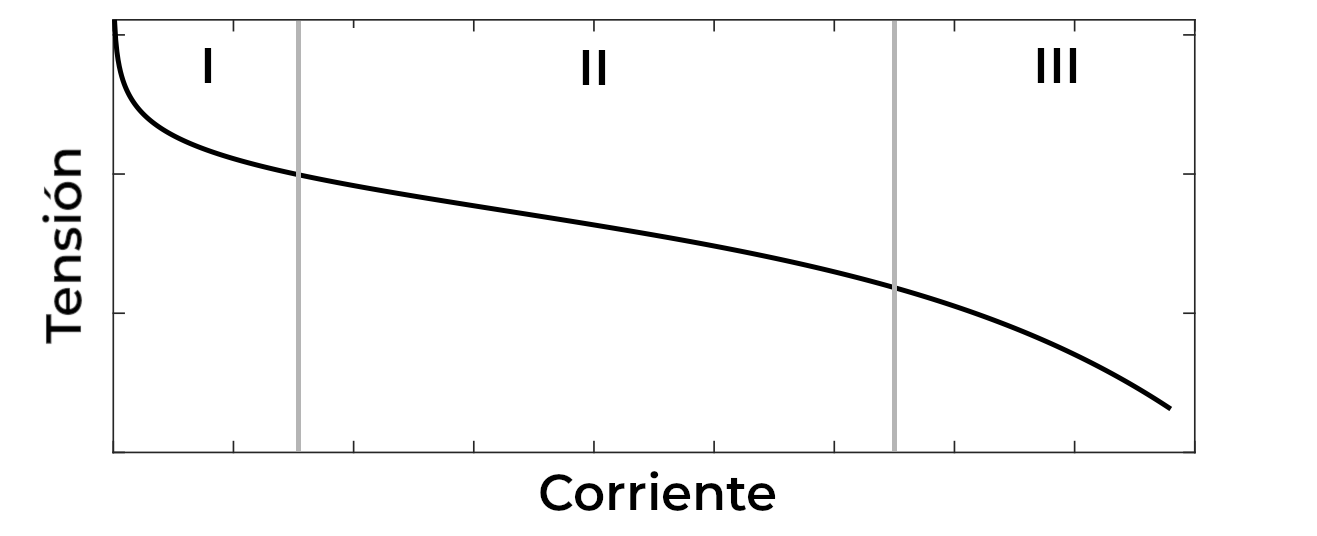
\includegraphics[scale=0.7]{Imagenes/Curva V-I Celda.png}
    \caption{Curva de tensión vs. corriente típica de una celda de combustible tipo PEM (Placeholder).}
    \label{V-I_celda}
\end{figure}

En esta curva se pueden señalar tres regiones de pérdidas bien marcadas: la región de \textbf{pérdidas de activación} cerca de corriente nula, seguida por la región de \textbf{pérdidas óhmicas}, y finalmente, acercándose a la máxima corriente, la región de \textbf{pérdidas de concentración}. Estas pérdidas se dan por algunas irreversibilidades de las reacciones que ocurren en la celda, que la alejan de su comportamiento ideal. A continuación se detallan estos componentes de la curva, obteniendo sus ecuaciones correspondientes.\\

\begin{enumerate}
    \bfseries \item Región de Pérdidas de Activación\\
    \normalfont Hola

    \bfseries \item Región de Pérdidas Óhmicas\\
    \normalfont Hola

    \bfseries \item Región de Pérdidas de Concentración\\
    \normalfont Hola
\end{enumerate}

\subsubsection{Emulador de Celdas de Combustible}

Hola\\